% !TeX root = RJwrapper.tex
\title{gdpR: An R Package for studying differentially private algorithms}


\author{by Jordan A. Awan, Kevin Eng, Robin Gong, Nianqiao Phyllis Ju, and Vinayak A. Rao}

\maketitle

\abstract{%
This paper serves as a reference and introduction on using the \(gdpR\) R package. The goal of this package is to provide some tools for exploring the impact of different privacy regimes on a Bayesian analysis. A strength of this framework is the ability to target the exact posterior in settings where the likelihood is too complex to analytically express.
}

\hypertarget{introduction}{%
\section{Introduction}\label{introduction}}

(cliche\ldots)
The ease and pervasiveness of modern data collection technologies has raised
concerns about data privacy. (Dwork and Roth 2013) introduced the differential privacy
framework as a means to rigorously define privacy.

\hypertarget{using}{%
\section{\texorpdfstring{Using \CRANpkg{gdpR}}{Using }}\label{using}}

The package is structured around the two functions \texttt{gdp\_sample} and
\texttt{new\_privacy}. The first function is used to draw samples from the
posterior. The second function is used to create the privacy model. Since the
input to these functions are R functions, there is a great deal of freedom
left up to user. The next two sections describe in detail the inputs into
these functions and highlight some considerations that should be taken
into account in order avoid slow or unexpected behavior.

\hypertarget{sampling}{%
\subsection{Sampling}\label{sampling}}

The main function in \pkg{gdpR} is the \texttt{gdp\_sample} function. The call
signature of the function is:

\begin{verbatim}
gdp_sample(data_model, sdp, nobs, init_par, niter = 2000, warmup = floor(niter / 2),
           chains = 1, varnames = NULL)
\end{verbatim}

The three required inputs into \texttt{gdp\_sample} function are the privacy model (\texttt{data\_model}), the value
of the observed privatized statistic (\texttt{sdp}), and the total number of observations
in the complete data (\texttt{nobs}) {[}MAKE SURE NOTATION IS INTRODUCED{]}. The \CRANpkg{gdpR}
package is best suited for problems where the complete data can be represented in
tabular form. This is because internally, it is represented as a matrix.

The optional arguments are the number of mcmc draws (\texttt{niter}), the
burn in period (\texttt{warmup}), number of chains (\texttt{chains}) and character
vector that names the parameters. Running multiple chains can be done in parallel
using the \CRANpkg{furrr} package. Additionally, progress can be monitored
using the \CRANpkg{progressr} package.

The \texttt{data\_model} input is a \texttt{privacy}
object that can be constructed using the \texttt{new\_privacy} constructor. The
process of constructing a \texttt{privacy} object will be discussed in the next section.

\hypertarget{privacy-model}{%
\subsection{Privacy Model}\label{privacy-model}}

Creating a privacy model is done using the \texttt{new\_privacy} constructor. The
main arguments consist of the four components as outlined in the methodology
section.

\begin{verbatim}
new_privacy(post_smpl = NULL, lik_smpl = NULL, ll_priv_mech = NULL,
            st_calc = NULL, add = FALSE, npar = NULL)
\end{verbatim}

The internal implementation of the DA algorithm in \texttt{gdp\_sample} requires
some care in how each component in constructed.

\begin{itemize}
\item
  \texttt{lik\_smpl} is an R function that samples from the likelihood. Its
  call signature should be \texttt{lik\_smpl(theta)} where \texttt{theta} is a vector
  representing the likelihood model parameters being estimated. This function
  must work with the supplied initial parameter provide in the \texttt{init\_par}
  argument of \texttt{gdp\_sample}. The sampler need not be vectorized and vectorizing
  the sampler will not add any speed benefits.
\item
  \texttt{post\_smpl} is a function which represents the posterior sampler. It should
  have the call signature \texttt{post\_smpl(dmat,\ theta)}. Where \texttt{dmat} is the
  complete data. This sampler can be generated by wrapping mcmc samplers generated from other R packages
  (e.g.~\CRANpkg{rstan}, \CRANpkg{fmcmc}, \CRANpkg{adaptMCMC}).
  If using this approach, it is recommended to avoid using packages such as \CRANpkg{mcmc}
  whose implementation clashes with \texttt{gdp\_sample}. In the case of \CRANpkg{mcmc},
  the Metropolis-Hastings loop is implemented in C which incurs a very large overhead
  in \texttt{gdp\_sample} since it is reinitialized every iteration. In general, repeatedly calling
  an R function that hooks into C code is slow. (NOT QUITE ACCURATE FIX LATER)
\item
  \texttt{ll\_priv\_mech} is an R function that represents the log-likelihood of
  \(\eta(s_{sdp} \mid x)\). The function can output the log likelihood
  up to an additive constant.
\item
  \texttt{st\_calc} is an R function which calculates the summary statistic. The optional
  argument \texttt{add} is a flag which represents whether \(T\) is additive or not.
\end{itemize}

\hypertarget{examples}{%
\section{Examples}\label{examples}}

\hypertarget{x2-contingency-table}{%
\subsection{2x2 Contingency Table}\label{x2-contingency-table}}

A common procedure when analyzing contingency tables is to estimate the
odds ratio. Something something about safetab to connect back to DP (dont forget citation!).
As a demonstration, we analyze the UC Berkeley admissions data, which is often
used as an illustrative example of Simpson's paradox. The question is whether
the data suggest there is bias against females during the college admissions
process. Below is a table of the aggregate admissions result from six departments based on sex.

\begin{table}[!h]

\centering
\begin{tabular}[t]{lrr}
\toprule
  & Male & Female\\
\midrule
Admitted & 1198 & 557\\
Rejected & 1493 & 1278\\
\bottomrule
\end{tabular}
\centering
\begin{tabular}[t]{lrr}
\toprule
  & Male & Female\\
\midrule
Admitted & 1135 & 473\\
Rejected & 1511 & 1438\\
\bottomrule
\end{tabular}
\end{table}

Below we walk through the process of defining a privacy model.

\begin{enumerate}
\def\labelenumi{\arabic{enumi}.}
\item
  \texttt{lik\_smpl}: Conditional on the table total, the table counts follow a multinomial
  distribution. We can easily draw from this distribution using the
  \texttt{rmultinom} function in the \texttt{base} stats package. Note, in this example,
  the return value of one sample from \texttt{rmultinom} is a \(4 \times 1\) matrix. In order to
  conform with \texttt{gdp\_sample} we must convert the matrix to a vector.

\begin{verbatim}
lik_smpl <- function(theta) {
  c(rmultinom(1, 4526, theta))
}
\end{verbatim}
\item
  \texttt{post\_smpl}: Given confidential data \(X\) we can derive the posterior analytically
  using a Dirichlet prior. In this example, we use a flat prior which
  corresponds to Dirch(1) distribution. A sample from the Dirichlet distribution
  can be generated using the gamma distribution via the following relation (INSERT)

\begin{verbatim}
post_smpl <- function(dmat, theta) {
  x <- c(dmat)
  t1 <- rgamma(length(theta), x + 1, 1)
  t1/sum(t1)
}
\end{verbatim}
\item
  \texttt{st\_calc}: The complete data can be represented in two ways. Micro vs cell totals.
  (what section to introduce?) This function must return a vector.

\begin{verbatim}
st_calc <- function(dmat) {
  c(dmat)
}
\end{verbatim}
\item
  \texttt{ll\_priv\_mech}: Privacy Mechanism
  Guassian white noise is added to each cell total. Hence given
  confidential data \((n_{11}, n_{22}, n_{12}, n_{21})\)
  \[
  \eta(s_{dp} \mid x) = \prod \phi(s_{sd}; n_{ij}, 100^2)
  \]

\begin{verbatim}
ll_priv_mech <- function(sdp, x) {
  dnorm(sdp - x, mean = 0, sd = 100, log = TRUE)
}
\end{verbatim}
\end{enumerate}

Once privacy model has been defined we can run \texttt{gdp\_sample}

\begin{verbatim}
library(DPloglin)
dmod <- new_privacy(post_smpl = post_smpl,
                    lik_smpl = lik_smpl,
                    ll_priv_mech = ll_priv_mech,
                    st_calc = st_calc,
                    add = FALSE,
                    npar = 4)

gdp_out <- gdp_sample(dmod,
                  sdp = c(adm_prv),
                  nobs = 1,
                  niter = 6000,
                  warmup = 1000,
                  chains = 1,
                  init_par = rep(.25,4),
                  varnames = c("pi_11", "pi_21", "pi_12", "pi_22"))
\end{verbatim}

results can be quickly summarized using the \texttt{summary} function

\begin{verbatim}
#> # A tibble: 4 x 10
#>   variable  mean median     sd    mad     q5   q95  rhat ess_bulk ess_tail
#>   <chr>    <num>  <num>  <num>  <num>  <num> <num> <num>    <num>    <num>
#> 1 pi_11    0.248  0.249 0.0258 0.0256 0.203  0.288  1.00     96.1     183.
#> 2 pi_21    0.335  0.335 0.0238 0.0239 0.293  0.373  1.01    107.      157.
#> 3 pi_12    0.102  0.101 0.0305 0.0321 0.0486 0.152  1.02     34.8     100.
#> 4 pi_22    0.316  0.316 0.0247 0.0256 0.275  0.356  1.00    119.      241.
\end{verbatim}

Diagnostic checks can be done using the \pkg{Bayesplot} package.

\begin{center}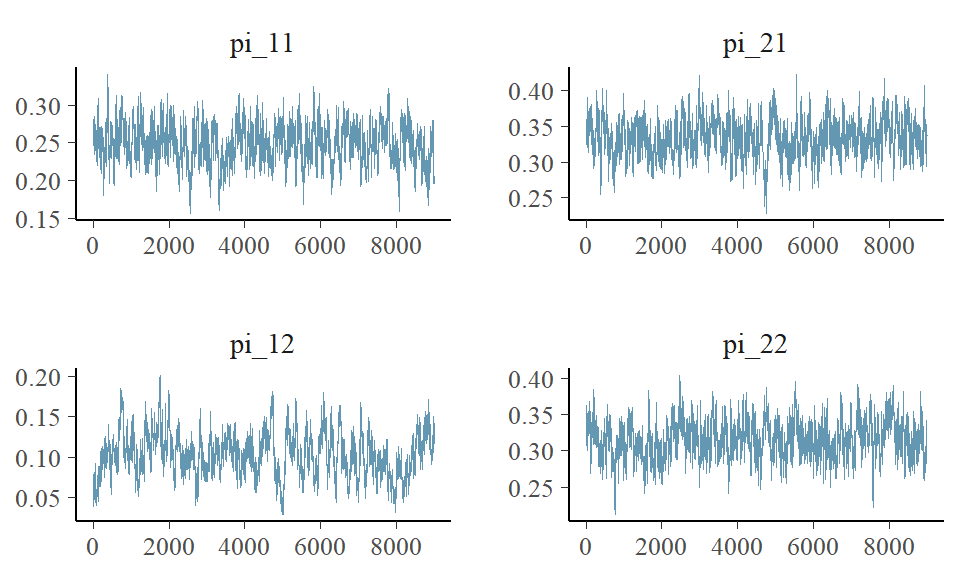
\includegraphics{dppaper_files/figure-latex/unnamed-chunk-12-1} \end{center}

log odds distribution

\begin{verbatim}
#>     2.5%      50%    97.5% 
#> 1.215316 2.321789 6.062528
\end{verbatim}

\begin{center}\includegraphics{dppaper_files/figure-latex/unnamed-chunk-13-1} \end{center}

(Insert gdp Analysis Here)

For clean data, a estimate for the odds ratio and a confidence interval
can be constructed using Woolf's method (i.e.~A wald confidence interval).
It uses the fact that the log of the odds ratio is approximately
normal for large sample sizes.
\[
\log\left(\dfrac{n_{11} \cdot n_{22}}{n_{12} \cdot n_{21}}\right) 
  \pm z_{\alpha/2}\sqrt{\dfrac{1}{n_{11}} + \dfrac{1}{n_{22}} + \dfrac{1}{n_{12}} + \dfrac{1}{n_{21}}}
\]

\begin{verbatim}
or_confint <- function(x, alpha) {
  or <- log(x[1] * x[4]/ (x[2] * x[3]))
  se <- sqrt(sum(1/x))
  c(or - qnorm(alpha/2) * se, or + qnorm(alpha/2) * se)
}

#clean data
exp(or_confint(x, .95))
\end{verbatim}

\begin{verbatim}
#> [1] 1.848471 1.833718
\end{verbatim}

\begin{verbatim}
#privitized data
exp(or_confint(sdp, .95))
\end{verbatim}

\begin{verbatim}
#> [1] 2.293115 2.274220
\end{verbatim}

\hypertarget{summary}{%
\section{Summary}\label{summary}}

This package is cool. You should install it.

\hypertarget{references}{%
\section*{References}\label{references}}
\addcontentsline{toc}{section}{References}

\hypertarget{refs}{}
\begin{CSLReferences}{1}{0}
\leavevmode\vadjust pre{\hypertarget{ref-Dwork2013}{}}%
Dwork, Cynthia, and Aaron Roth. 2013. {``The Algorithmic Foundations of Differential Privacy.''} \emph{Foundations and Trends{\textregistered} in Theoretical Computer Science} 9 (3-4): 211--407. \url{https://doi.org/10.1561/0400000042}.

\end{CSLReferences}

\bibliography{RJreferences.bib}

\address{%
Jordan A. Awan\\
Purdue University\\%
Department of Statistics\\ West Lafayette, IN 47907\\
%
\url{https://www.britannica.com/animal/quokka}\\%
%
\href{mailto:jawan@purdue.edu}{\nolinkurl{jawan@purdue.edu}}%
}

\address{%
Kevin Eng\\
Rutgers University\\%
Department of Statistics\\ Piscataway, NJ 08854\\
%
\url{https://www.britannica.com/animal/quokka}\\%
%
\href{mailto:ke157@stat.rutgers.edu}{\nolinkurl{ke157@stat.rutgers.edu}}%
}

\address{%
Robin Gong\\
Rutgers University\\%
Department of Statistics\\ Piscataway, NJ 08854\\
%
\url{https://www.britannica.com/animal/quokka}\\%
%
\href{mailto:ruobin.gong@rutgers.edu}{\nolinkurl{ruobin.gong@rutgers.edu}}%
}

\address{%
Nianqiao Phyllis Ju\\
Purdue University\\%
Department of Statistics\\ West Lafayette, IN 47907\\
%
\url{https://www.britannica.com/animal/quokka}\\%
%
\href{mailto:nianqiao@purdue.edu}{\nolinkurl{nianqiao@purdue.edu}}%
}

\address{%
Vinayak A. Rao\\
Purdue University\\%
Department of Statistics\\ West Lafayette, IN 47907\\
%
\url{https://www.britannica.com/animal/quokka}\\%
%
\href{mailto:varao@purdue.edu}{\nolinkurl{varao@purdue.edu}}%
}
